\documentclass{article}
\usepackage[T1]{fontenc}
\usepackage[utf8]{inputenc}
\usepackage{amssymb}
\usepackage{pythonhighlight}
\usepackage{tikz}
\usepackage{amsmath}
\usepackage[a4paper, left=40mm, right=40mm, top=30mm, bottom=30mm]{geometry}
\usepackage[indent=0pt]{parskip}
\usepackage{graphicx}
\usepackage{subfig}
\usepackage{subcaption}
\usepackage{hyperref}
\usepackage{float}
\usepackage{csquotes}
\usepackage[backend=biber]{biblatex}
\addbibresource{matrices.bib}
\graphicspath{ {../images/} }
    
\title{Metody numeryczne - projekt 2 - Układy równań liniowych}
\author{Jerzy Szyjut, numer albumu: 193064}
\date{20.04.2024r.}

\begin{document}

\maketitle

\begin{section}{Wstęp}
    \subsection{Układy równań liniowych}
    Układ równań liniowych to zbiór równań postaci:
    \begin{equation}
        Ax = b
    \end{equation}
    Gdzie dane są macierz kwadratowa A i wektor b, a szukany jest wektor x.
    Powyższe równanie macierzowe można zapisać w postaci równań:
    \begin{equation*}
        \begin{cases}
            a_{11}x_1 + a_{12}x_2 + \ldots + a_{1n}x_n = b_1 \\
            a_{21}x_1 + a_{22}x_2 + \ldots + a_{2n}x_n = b_2 \\
            \hspace{27 mm} \vdots \\
            a_{n1}x_1 + a_{n2}x_2 + \ldots + a_{nn}x_n = b_n
        \end{cases}
    \end{equation*}

    \subsection{Metody bezpośrednie rozwiązywania układów równań liniowych}
    Najprostszym sposobem rozwiązania układu równań liniowych jest metoda eliminacji Gaussa.
    Metoda ta polega na przekształceniu macierzy A do postaci macierzy trójkątnej górnej, a następnie
    rozwiązaniu układu równań za pomocą algorytmu podstawiania wstecz. Metoda ta ma złożoność obliczeniową
    $O(n^3) + O(mn^2)$ \cite{wyklad1}.

    Kolejną metodą rozwiązywania układów równań liniowych jest faktoryzacja LU. Metoda ta polega na
    rozkładzie macierzy A na iloczyn dwóch macierzy L i U, gdzie L to macierz trójkątna dolna, a U to
    macierz trójkątna górna, tak że $LUx = b$. Tworzymy wektor pomocniczy $y = Ux$
    Następnie rozwiązujemy dwa układy równań liniowych:
    \begin{align*}
        Ly = b \\
        Ux = y
    \end{align*}

    W metodzie faktoryzacji LU zastosowano eliminację Gaussa, ale przez rozłożenie macierzy A na dwie
    macierze trójkątne L i U, algorytm podstawiania wstecz ma złożoność obliczeniową $O(n^2)$\cite{wyklad1}, a nie $O(n^3)$.
    W całości metoda faktoryzacji LU ma złożoność obliczeniową $O(n^3)$ \cite{wyklad1}.

    Dodatkowo w metodzie faktoryzacji LU czasochłonne rozkładanie macierzy A na dwie macierze L i U
    wykonuje się tylko raz i można wielokrotnie rozwiązywać układ równań liniowych dla różnych wektorów b.

    \subsection{Metody iteracyjne rozwiązywania układów równań liniowych}
    Metody iteracyjne polegają na rozwiązaniu układu równań liniowych poprzez iteracyjne przybliżanie
    rozwiązania. W każdej iteracji obliczane jest nowe przybliżenie rozwiązania, które jest coraz bliższe
    rzeczywistemu rozwiązaniu. Metody iteracyjne są zazwyczaj mniej dokładne niż metody bezpośrednie, ale
    pozwalają na rozwiązanie dużych układów równań liniowych w krótszym czasie przy większym marginesie błędu.

    Przykładem metody iteracyjnej jest metoda Jacobiego. Metoda ta polega na podziale macierzy A na
    macierz diagonalną D, macierz trójkątną dolną L i macierz trójkątną górną U, tak że $A = D - L - U$.
    Następnie iteracyjnie obliczane jest nowe przybliżenie rozwiązania $x^{(k+1)}$ na podstawie poprzedniego
    przybliżenia $x^{(k)}$:
    \begin{equation}
        x^{(k+1)} = D^{-1}(L + U)x^{(k)} + D^{-1}b
    \end{equation} \cite{wyklad2}

    Kolejną metodą iteracyjną jest metoda Gaussa-Seidla, która działa w bardzo zbliżony sposób do metody
    Jacobiego, ale w każdej iteracji korzysta z najnowszych wartości $x^{(k+1)}$. Metodę Gaussa-Seidla
    można opisać równaniem:
    \begin{equation}
        x^{(k+1)} = (D - L)^{-1}Ux^{(k)} + (D - L)^{-1}b
    \end{equation} \cite{wyklad2}
    Dzięki temu metoda Gaussa-Seidla zazwyczaj szybciej zbiega do rozwiązania niż metoda Jacobiego.

    \subsection{Wektor residuum}
    W przypadku metod iteracyjnych, wskaźnikiem jakości rozwiązania układu równań liniowych w obecnej iteracji
    jest wektor residuum. Wektor residuum to wektor, który można uzyskać wzorem:
    \begin{equation}
        res = Ax - b
    \end{equation}
    Wartość wektora residuum mówi o tym, jak bardzo rozwiązanie uzyskane w danej iteracji różni się od
    rzeczywistego rozwiązania. Im mniejsza wartość wektora residuum, tym lepsze przybliżenie rozwiązania.
    Gdy norma wektora residuum jest mniejsza od zadanego progu błędu, można uznać, że rozwiązanie jest
    wystarczająco dokładne. Normę wektora oblicza się wzorem:
    \begin{equation}
        ||res|| = \sqrt{\sum_{i=1}^{n}res_i^2}
    \end{equation}
\end{section}

\begin{section}{Metody Jacobiego i Gaussa-Seidla dla macierzy z silną dominacją w wierszach}
    \label{sec:1}
    \subsection{Macierz A i wektor b}
    Macierze A i wektor b użyte dla algorytmów w tej sekcji to:
    \begin{equation}
        A = \begin{bmatrix}
            5 & -1 & -1 & 0 & \cdots & 0 & 0 & 0 & 0 \\
            -1 & 5 & -1 & -1 & \cdots & 0 & 0 & 0 & 0 \\
            -1 & -1 & 5 & -1 & \cdots & 0 & 0 & 0 & 0 \\
            0 & -1 & -1 & 5 & \cdots & 0 & 0 & 0 & 0 \\
            \vdots & \vdots & \vdots & \vdots & \ddots & \vdots & \vdots & \vdots & \vdots \\
            0 & 0 & 0 & 0 & \cdots & 5 & -1 & -1 & 0 \\
            0 & 0 & 0 & 0 & \cdots & -1 & 5 & -1 & -1 \\
            0 & 0 & 0 & 0 & \cdots & -1 & -1 & 5 & -1 \\
            0 & 0 & 0 & 0 & \cdots & 0 & -1 & -1 & 5 \\
        \end{bmatrix}
    \end{equation}
    \begin{equation}
        b = \begin{bmatrix}
            sin(3 \cdot 1) \\
            sin(3 \cdot 2) \\
            sin(3 \cdot 3) \\
            \vdots \\
            sin(3 \cdot n)
        \end{bmatrix}
    \end{equation}
    Macierz A ma rozmiar $n \times n$, gdzie $n = 964$, a wektor b ma długość $n$.
    
    \subsection{Porównanie metod Jacobiego i Gaussa-Seidla}
    \begin{center}
        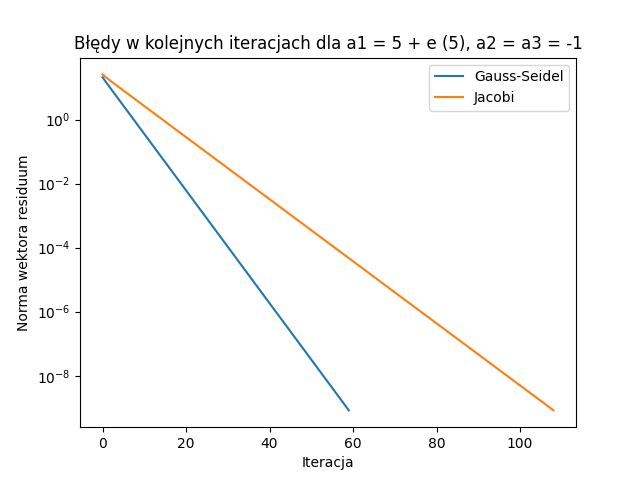
\includegraphics[width=0.8\textwidth]{bledy_zbiezne.png}
    \end{center}
    Na powyższym wykresie przedstawiono zmiany wartości normy wektora residuum w zależności od liczby iteracji
    dla metod Jacobiego i Gaussa-Seidla. Jak widać, metoda Gaussa-Seidla zbiega do rozwiązania znacznie szybciej
    niż metoda Jacobiego. Dla zadanego progu błędu $\epsilon = 10^{-9}$ metoda Gaussa-Seidla osiąga zbieżność w 42
    iteracjach, podczas gdy metoda Jacobiego osiąga zbieżność w 70 iteracjach.
    \begin{table}[H]
        \centering
        \begin{tabular}{|c|c|c|c|}
            \hline
            Metoda & Liczba iteracji & Czas obliczeń [s] & Norma wektora residuum \\
            \hline
            Jacobiego & $70$ & $11.79$ & $8.58\cdot10^{-10}$ \\
            Gaussa-Seidla & $42$ & $8.46$ & $6.66\cdot10^{-10}$ \\
            \hline
        \end{tabular}
        \caption{Porównanie liczby iteracji, czasu obliczeń i normy wektora residuum dla metod Jacobiego i Gaussa-Seidla}
    \end{table}
    Jako, że metoda Gaussa-Seidla wykonuje zbliżone obliczenia do metody Jacobiego, to mniejsza liczba iteracji 
    będzie oznaczała krótszy czas obliczeń.
\end{section}

\begin{section}{Metody Jacobiego i Gaussa-Seidla dla macierzy rozbieżnej}
    \subsection{Macierz A i wektor b}
    Macierze A i wektor b użyte dla algorytmów w tej sekcji to:
    \begin{equation}
        A = \begin{bmatrix}
            3 & -1 & -1 & 0 & \cdots & 0 & 0 & 0 & 0 \\
            -1 & 3 & -1 & -1 & \cdots & 0 & 0 & 0 & 0 \\
            -1 & -1 & 3 & -1 & \cdots & 0 & 0 & 0 & 0 \\
            0 & -1 & -1 & 3 & \cdots & 0 & 0 & 0 & 0 \\
            \vdots & \vdots & \vdots & \vdots & \ddots & \vdots & \vdots & \vdots & \vdots \\
            0 & 0 & 0 & 0 & \cdots & 3 & -1 & -1 & 0 \\
            0 & 0 & 0 & 0 & \cdots & -1 & 3 & -1 & -1 \\
            0 & 0 & 0 & 0 & \cdots & -1 & -1 & 3 & -1 \\
            0 & 0 & 0 & 0 & \cdots & 0 & -1 & -1 & 3 \\
        \end{bmatrix}
    \end{equation}
    \begin{equation}
        b = \begin{bmatrix}
            sin(3 \cdot 1) \\
            sin(3 \cdot 2) \\
            sin(3 \cdot 3) \\
            \vdots \\
            sin(3 \cdot n)
        \end{bmatrix}
    \end{equation}
    Macierz A ma rozmiar $n \times n$, gdzie $n = 964$, a wektor b ma długość $n$.

    \subsection{Porównanie metod Jacobiego i Gaussa-Seidla}
    \begin{center}
        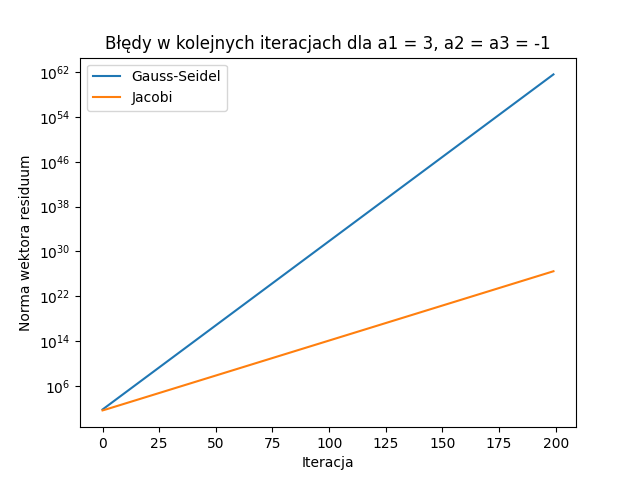
\includegraphics[width=0.8\textwidth]{bledy_rozbiezne.png}
    \end{center}
    Na powyższym wykresie przedstawiono zmiany wartości normy wektora residuum w zależności od liczby iteracji
    dla metod Jacobiego i Gaussa-Seidla. Jak widać, norma wektora residuum dla obu metod zbiega do nieskończoności.
    Wynika to z faktu, że macierz macierz $T = D^{-1}(L + U)$ ma promień spektralny (największa wartość własna - eigenvalue)
    większy od 1\cite{wyklad3}. W takim przypadku metody iteracyjne nie zbiegają do rozwiązania.

    \begin{table}[H]
        \centering
        \begin{tabular}{|c|c|c|c|}
            \hline
            Metoda & Liczba iteracji & Czas obliczeń [s] & Norma wektora residuum \\
            \hline
            Jacobiego & $100$ & $17.47$ & $1.25\cdot10^{10}$ \\
            Gaussa-Seidla & $100$ & $20.08$ & $9.74\cdot10^{27}$ \\
            \hline
        \end{tabular}
        \caption{Porównanie liczby iteracji, czasu obliczeń i normy wektora residuum dla metod Jacobiego i Gaussa-Seidla}
    \end{table}
    Jak widać, obie metody zakończyły swoje działanie po 100 iteracjach, co jest maksymalną liczbą iteracji w moim programie.

\end{section}

\begin{section}{Faktoryzacja LU}
    Macierzy przedstawioną w poprzedniej sekcji można poddać faktoryzacji LU, tam gdzie metody Jacobiego i Gaussa-Seidla
    zawiodły.
    \begin{table}[H]
        \centering
        \begin{tabular}{|c|c|c|c|}
            \hline
            Metoda & Czas obliczeń [s] & Norma wektora residuum \\
            \hline
            Faktoryzacja LU & $39.13$ & $2.36\cdot10^{-13}$ \\
            \hline
        \end{tabular}
        \caption{Wyniki faktoryzacji LU dla macierzy rozbieżnej}
    \end{table}
    Jak widać, faktoryzacja LU pozwoliła na uzyskanie dokładnego rozwiązania układu równań liniowych, jednak
    czas obliczeń był znacznie dłuższy niż dla metod iteracyjnych.
\end{section}

\begin{section}{Porównanie metod Jacobiego, Gaussa-Seidla i faktoryzacji LU}
    Metody Jacobiego i Gaussa-Seidla i faktoryzacji LU zostały uruchomione dla macierzy z sekcji 
    \hyperref[sec:1]{Metody Jacobiego i Gaussa-Seidla dla macierzy z silną dominacją w wierszach}.
    Rozmiary macierzy i wektora $n$ należą do zbioru $\{500, 1000, 2000, 3000, 4000\}$.

    \begin{center}
        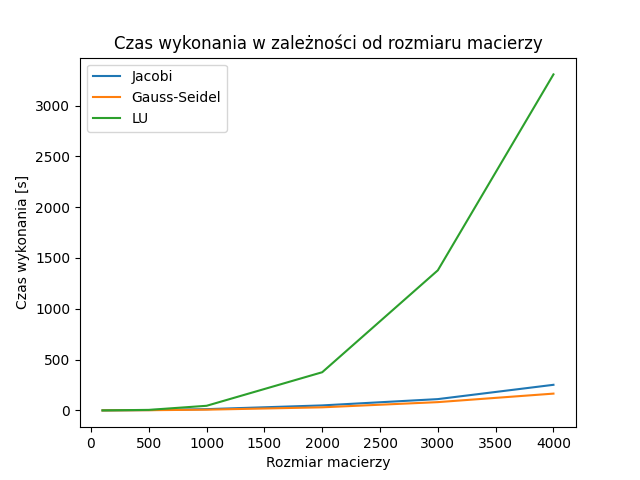
\includegraphics[width=0.8\textwidth]{czas_wykonania.png}
    \end{center}

    \begin{table}
        \centering
        \begin{tabular}{|c|c|c|c|c|}
            \hline
            Metoda & Liczba iteracji & Czas obliczeń [s] & Norma wektora residuum \\
            \hline
            Jacobiego & $69$ & $0.15$ & $9.11\cdot10^{-10}$ \\
            Gaussa-Seidla & $41$ & $0.09$ & $9.11\cdot10^{-10}$ \\
            Faktoryzacja LU & $1$ & $0.06$ & $7.93\cdot10^{-16}$ \\
            \hline
        \end{tabular}
        \caption{Porównanie dla $n = 100$}
    \end{table}

    \begin{table}
        \centering
        \begin{tabular}{|c|c|c|c|c|}
            \hline
            Metoda & Liczba iteracji & Czas obliczeń [s] & Norma wektora residuum \\
            \hline
            Jacobiego & $71$ & $3.30$ & $8.24\cdot10^{-10}$ \\
            Gaussa-Seidla & $42$ & $1.90$ & $8.24\cdot10^{-10}$ \\
            Faktoryzacja LU & $1$ & $5.13$ & $1.78\cdot10^{-15}$ \\
            \hline
        \end{tabular}
        \caption{Porównanie dla $n = 500$}
    \end{table}

    \begin{table}
        \centering
        \begin{tabular}{|c|c|c|c|c|}
            \hline
            Metoda & Liczba iteracji & Czas obliczeń [s] & Norma wektora residuum \\
            \hline
            Jacobiego & $69$ & $12.34$ & $9.03\cdot10^{-10}$ \\
            Gaussa-Seidla & $40$ & $7.25$ & $7.25\cdot10^{-10}$ \\
            Faktoryzacja LU & $1$ & $45.42$ & $2.50\cdot10^{-15}$ \\
            \hline
        \end{tabular}
        \caption{Porównanie dla $n = 1000$}
    \end{table}

    \begin{table}
        \centering
        \begin{tabular}{|c|c|c|c|c|}
            \hline
            Metoda & Liczba iteracji & Czas obliczeń [s] & Norma wektora residuum \\
            \hline
            Jacobiego & $70$ & $49.15$ & $9.62\cdot10^{-10}$ \\
            Gaussa-Seidla & $42$ & $30.34$ & $9.62\cdot10^{-10}$ \\
            Faktoryzacja LU & $1$ & $375.68$ & $3.53\cdot10^{-15}$ \\
            \hline
        \end{tabular}
        \caption{Porównanie dla $n = 2000$}
    \end{table}

    \begin{table}
        \centering
        \begin{tabular}{|c|c|c|c|c|}
            \hline
            Metoda & Liczba iteracji & Czas obliczeń [s] & Norma wektora residuum \\
            \hline
            Jacobiego & $70$ & $111.21$ & $9.99\cdot10^{-10}$ \\
            Gaussa-Seidla & $42$ & $81.47$ & $9.99\cdot10^{-10}$ \\
            Faktoryzacja LU & $1$ & $1378.66$ & $4.31\cdot10^{-15}$ \\
            \hline
        \end{tabular}
        \caption{Porównanie dla $n = 3000$}
    \end{table}

    \begin{table}
        \centering
        \begin{tabular}{|c|c|c|c|c|}
            \hline
            Metoda & Liczba iteracji & Czas obliczeń [s] & Norma wektora residuum \\
            \hline
            Jacobiego & $69$ & $251.88$ & $8.00\cdot10^{-10}$ \\
            Gaussa-Seidla & $40$ & $165.24$ & $8.00\cdot10^{-10}$ \\
            Faktoryzacja LU & $1$ & $3306.43$ & $4.93\cdot10^{-15}$ \\
            \hline
        \end{tabular}
        \caption{Porównanie dla $n = 4000$}
    \end{table}

    Z powyższych tabel wynika, że liczba iteracji dla metod Jacobiego i Gaussa-Seidla jest zbliżona dla
    macierzy o dowolnym rozmiarze $n$, natomiast iteracje były dłuższe dla większych macierzy.

    Faktoryzacja LU nie skaluje się tak dobrze jak metody iteracyjne, co wynika z faktu, że faktoryzacja LU
    ma złożoność obliczeniową $O(n^3)$. 
\end{section}

\begin{section}{Wnioski}
    Chociaż metoda faktoryzacji LU daje dokładne wyniki, wymaga znacznie więcej czasu obliczeń niż metody iteracyjne,
    w których można kontrolować dokładność rozwiązania przez zdefiniowanie progu błędu. Dla większych macierzy
    faktoryzacja LU jest niepraktyczna przez słabą skalowalność. 

    Jednak metody iteracyjne czasem zawodzą i nie zbiegają do wyniku, więc w przypadku gdy wykryje się rozbieżność,
    pozostaje nam faktoryzacja LU, która zawsze zwróci rozwiązanie.
\end{section}

\printbibliography

\end{document}
